%-------------------------------------------------------------------------------
% This file provides a skeleton ATLAS note.
% \pdfinclusioncopyfonts=1
% This command may be needed in order to get \ell in PDF plots to appear. Found in
% https://tex.stackexchange.com/questions/322010/pdflatex-glyph-undefined-symbols-disappear-from-included-pdf
%-------------------------------------------------------------------------------
% Specify where ATLAS LaTeX style files can be found.
\newcommand*{\ATLASLATEXPATH}{latex/}
% Use this variant if the files are in a central location, e.g. $HOME/texmf.
% \newcommand*{\ATLASLATEXPATH}{}
%-------------------------------------------------------------------------------
\documentclass[NOTE, atlasdraft=true, texlive=2016, USenglish]{\ATLASLATEXPATH atlasdoc}
% The language of the document must be set: usually UKenglish or USenglish.
% british and american also work!
% Commonly used options:
%  atlasdraft=true|false This document is an ATLAS draft.
%  texlive=YYYY          Specify TeX Live version (2016 is default).
%  coverpage             Create ATLAS draft cover page for collaboration circulation.
%                        See atlas-draft-cover.tex for a list of variables that should be defined.
%  cernpreprint          Create front page for a CERN preprint.
%                        See atlas-preprint-cover.tex for a list of variables that should be defined.
%  NOTE                  The document is an ATLAS note (draft).
%  PAPER                 The document is an ATLAS paper (draft).
%  CONF                  The document is a CONF note (draft).
%  PUB                   The document is a PUB note (draft).
%  BOOK                  The document is of book form, like an LOI or TDR (draft)
%  txfonts=true|false    Use txfonts rather than the default newtx
%  paper=a4|letter       Set paper size to A4 (default) or letter.

%-------------------------------------------------------------------------------
% Extra packages:
\usepackage{\ATLASLATEXPATH atlaspackage}
% Commonly used options:
%  biblatex=true|false   Use biblatex (default) or bibtex for the bibliography.
%  backend=bibtex        Use the bibtex backend rather than biber.
%  subfigure|subfig|subcaption  to use one of these packages for figures in figures.
%  minimal               Minimal set of packages.
%  default               Standard set of packages.
%  full                  Full set of packages.
%-------------------------------------------------------------------------------
% Style file with biblatex options for ATLAS documents.
\usepackage{\ATLASLATEXPATH atlasbiblatex}

% Package for creating list of authors and contributors to the analysis.
\usepackage{\ATLASLATEXPATH atlascontribute}

% Useful macros
\usepackage{\ATLASLATEXPATH atlasphysics}
\usepackage{siunitx}
% See doc/atlas_physics.pdf for a list of the defined symbols.
% Default options are:
%   true:  journal, misc, particle, unit, xref
%   false: BSM, heppparticle, hepprocess, hion, jetetmiss, math, process, other, texmf
% See the package for details on the options.

% Files with references for use with biblatex.
% Note that biber gives an error if it finds empty bib files.
\addbibresource{pPbJetCalibrationNote.bib}
\addbibresource{bib/ATLAS.bib}
\addbibresource{bib/CMS.bib}
\addbibresource{bib/ConfNotes.bib}
\addbibresource{bib/PubNotes.bib}

% Paths for figures - do not forget the / at the end of the directory name.
\graphicspath{{logos/}{figures/}}

% Add you own definitions here (file pPbJetCalibrationNote-defs.sty).
\usepackage{pPbJetCalibrationNote-defs}
\setlength{\parindent}{4ex}
%-------------------------------------------------------------------------------
% Generic document information
%-------------------------------------------------------------------------------

% Title, abstract and document 
%-------------------------------------------------------------------------------
% This file contains the title, author and abstract.
% It also contains all relevant document numbers used for an ATLAS note.
%-------------------------------------------------------------------------------

% Title
\AtlasTitle{Calibration of the Heavy Ion Jet Collection in 2016 \SI{8.16}{\TeV} \textit{p}-Pb Collisions}

% Draft version:
% Should be 1.0 for the first circulation, and 2.0 for the second circulation.
% If given, adds draft version on front page, a 'DRAFT' box on top of each other page, 
% and line numbers.
% Comment or remove in final version.
\AtlasVersion{0.1}

% Abstract - % directly after { is important for correct indentation
\AtlasAbstract{%
Numerical inversion is performed on reconstructed and truth jets in MC to obtain the eta jet energy scale (EtaJES) corrections in 2016 proton-lead collisions at \SI{8.16}{\TeV}. The calibration summary plots are presented and a procedure for applying the calibration is shown, with intended use for the 2016 \SI{8.16}{\TeV} \textit{p}-Pb data. Applicability of the insitu-based cross-calibration between EMTopo and HI jets in 2015 \SI{5.02}{\TeV} \textit{pp} collisions to the 2016 \textit{p}-Pb data is also tested by studying the $p_{\text{T}}$ balance in vector boson + jet events in the 2016 data. Additional systematics on the cross-calibration are presented by comparing data to MC.
}

% Author - this does not work with revtex (add it after \begin{document})
% \author{The ATLAS Collaboration}

% Authors and list of contributors to the analysis
% \AtlasAuthorContributor also adds the name to the author list
% Include package latex/atlascontribute to use this
% Use authblk package if there are multiple authors, which is included by latex/atlascontribute
% \usepackage{authblk}
% Use the following 3 lines to have all institutes on one line
% \makeatletter
% \renewcommand\AB@affilsepx{, \protect\Affilfont}
% \makeatother
% \renewcommand\Authands{, } % avoid ``. and'' for last author
% \renewcommand\Affilfont{\itshape\small} % affiliation formatting
% \AtlasAuthorContributor{First AtlasAuthorContributor}{a}{Author's contribution.}
% \AtlasAuthorContributor{Second AtlasAuthorContributor}{b}{Author's contribution.}
% \AtlasAuthorContributor{Third AtlasAuthorContributor}{a}{Author's contribution.}
% \AtlasContributor{Fourth AtlasContributor}{Contribution to the analysis.}
% \author[a]{First Author}
% \author[a]{Second Author}
% \author[b]{Third Author}
% \affil[a]{One Institution}
% \affil[b]{Another Institution}

% If a special author list should be indicated via a link use the following code:
% Include the two lines below if you do not use atlasstyle:
% \usepackage[marginal,hang]{footmisc}
% \setlength{\footnotemargin}{0.5em}
% Use the following lines in all cases:
% \usepackage{authblk}
% \author{The ATLAS Collaboration%
% \thanks{The full author list can be found at:\newline
%   \url{https://atlas.web.cern.ch/Atlas/PUBNOTES/ATL-PHYS-PUB-2017-007/authorlist.pdf}}
% }

% ATLAS reference code, to help ATLAS members to locate the paper
\AtlasRefCode{GROUP-2017-XX}

% ATLAS note number. Can be an COM, INT, PUB or CONF note
% \AtlasNote{ATLAS-CONF-2017-XXX}
% \AtlasNote{ATL-PHYS-PUB-2017-XXX}
% \AtlasNote{ATL-COM-PHYS-2017-XXX}

% Author and title for the PDF file
\hypersetup{pdftitle={ATLAS document},pdfauthor={The ATLAS Collaboration}}
\AtlasAuthorContributor{Jeffrey C. Ouellette}{a}{fake background estimate.}
\affil[a]{University of Colorado Boulder}

%-------------------------------------------------------------------------------
% Content
%-------------------------------------------------------------------------------
\begin{document}

\maketitle

\tableofcontents

% List of contributors - print here or after the Bibliography.
%\PrintAtlasContribute{0.30}
%\clearpage

\begin{center}
\begin{table}
\resizebox{\linewidth}{!}{
\begin{tabular}{| l | r |}
	\hline
	Sample descriptor & \# Events\\ \hline \hline
	{\tiny \texttt{mc15\_pPb8TeV.42001*.Pythia8EvtGen\_A14NNPDF23LO\_jetjet\_JZ*R04.merge.AOD.e651*\_s3084\_s3153\_r9985\_r9647}} & {\tiny 40M} \\ \hline
	{\tiny \texttt{mc15\_pPb8TeV.42310*.Pythia8EvtGen\_A14NNPDF23LO\_gammajet\_DP*\_*.merge.AOD.e544*\_e5984\_d14**\_r9645\_r9647}} & {\tiny 6M} \\ \hline
%	{\tiny \texttt{mc15\_valid.42310*.Pythia8EvtGen\_A14NNPDF23LO\_gammajet\_DP*\_*.merge.AOD.e5709\_s3084\_r9160\_r9006}} & {\tiny 300k} \\ \hline
	{\tiny \texttt{mc15\_pPb8TeV.361106.PowhegPythia8EvtGen\_AZNLOCTEQ6L1\_Zee.merge.AOD.e643*\_d146*\_r10136\_r9647}} & {\tiny 470k} \\ \hline
  	{\tiny \texttt{mc15\_pPb8TeV.361107.PowhegPythia8EvtGen\_AZNLOCTEQ6L1\_Zmumu.merge.AOD.e643*\_d146*\_r10136\_r9647}} & {\tiny 375k} \\ \hline
\end{tabular}
}
\caption{MC samples used in deriving the EtaJES corrections and deriving additional uncertainties from the 2015 cross-calibration. The first entry is a signal-only dijet sample, whereas the remainder apply minbias data overlay.}
\label{tab:samples}
\end{table}
\end{center}

%-------------------------------------------------------------------------------
\section{Introduction}
\label{sec:intro}
%-------------------------------------------------------------------------------

The reconstruction of anti-$k_{\text{T}}$ jets is well-known to misestimate the jet energy scale and pseudorapidity. Here, a standard numerical inversion method is applied to the heavy ion jet algorithm to estimate the $\eta$-dependent jet energy scale in truth-matched MC \cite{ATL-COM-PHYS-2014-795}. Further, to apply the \textit{in situ} corrections to the heavy ions jet algorithm \cite{ATLAS-CONF-2015-017}, the cross-calibration used in 2015 Pb+Pb collisions is applied to jets in the 2016 pPb collisions . The applicability of the cross-calibration is studied via momentum balance in events containing a vector boson and a jet. Although the original configuration of the cross-calibration applied the 2015 \textit{in situ} factors for EMTopo jets, a known issue between software releases led to different \textit{in situ} factors in 2016 \cite{ATLAS-CONF-2015-017}, so a new configuration has been created.\par
To derive the EtaJES corrections, 10 total jet $\pt$ samples were generated with Pythia 8, with 5 slices per beam direction. In checking the cross-calibration, a combination of Pythia 8 $\gamma$ + jet, $Z\rightarrow\ee$, and $Z\rightarrow\mumu$ events were used. A complete list of the samples used can be found in Table \ref{tab:samples}.


%-------------------------------------------------------------------------------
\section{Reconstruction of jets}
\label{sec:reconstruction}
%-------------------------------------------------------------------------------

The anti-$k_{\text{T}}$ heavy ion jet algorithm works differently than the standard EMTopo algorithm, which is well understood in \textit{pp} collisions \cite{Cacciari:2008gp}. The heavy ion algorithm takes $\Delta\eta\times\Delta\phi=0.1\times0.1$ calorimeter towers as input, subtracting the average energy from identified jets. This allows the underlying event energy to be uniformly subtracted away. While used primarily for large nuclear systems with significant underlying events such as Pb+Pb, the algorithm can be also applied to small systems, such as \textit{p}+Pb, as is presented here. A similar discussion can be found in the 2015 calibration \cite{ATL-COM-PHYS-2016-101}.\par
\subsection{Jet selection criteria}
For deriving the EtaJES calibration, jets are reconstructed at the EM scale with anti-$k_{\text{T}}$ radii $R=0.2, 0.3, 0.4$. After satisfying the physicality condition (where jets must have an energy strictly greater than their mass), reconstructed jets must meet a jet cleaning criterion at the \texttt{LooseBad} level. Events affected by pile-up are skipped by selecting on a minimum $\pt$ quality ratio, which is defined as the ratio of the average $\pt$ between the 2 leading reconstructed jets and the leading truth jet. This ratio is selected to be less than 1.4. Additionally, truth jets must satisfy $\pt > \SI{7}{\GeV}$ and have an isolation of $\Delta R > 1.0$ from all other truth jets. Reconstructed jets are similarly required to have $\pt > \SI{7}{\GeV}$ and have an isolation of $\Delta R > 0.6$ from all other reconstructed jets. Matching is performed with $\Delta R < 0.3$ between truth and reconstructed jets.
\subsection{Hadronic Calorimeter cuts}
Lastly, a portion of the hadronic calorimeter end cap (referred to as the ``HEC'') was turned off during the entire 2016 \textit{p}+Pb data taking period. For this reason, jets within the disabled region, defined by $1.5<\eta<3.2$ and $-\pi<\phi<-\pi/2$, were selected against at both the truth and reconstructed level. Jets were also required to have additional $\Delta\eta, \Delta\phi \geq 0.2$ from the disabled region in order to avoid edge effects, although for analyses it is recommended to use $\Delta R$ equal to the jet cone size (e.g., $0.4$) to avoid edge effects.

%\subsection{\Antikt}

The \antikt algorithm with a radius parameter of $R=0.4$ is used to reconstruct jets with a four-momentum recombination scheme, using \topos as inputs. Jet energy is calibrated to the hadronic scale with the effect of \pileup removed

\subsection{\Topos}

Hadronic jets are reconstructed from calibrated three-dimensional \topos.
Clusters are constructed from calorimeter cells that are grouped together using a topological clustering algorithm.
These objects provide a three-dimensional representation of energy depositions in the calorimeter and implement a nearest-neighbour noise suppression algorithm.
The resulting \topos are classified as either electromagnetic or hadronic based on their shape, depth and energy density.
Energy corrections are then applied to the clusters in order to calibrate them to the appropriate energy scale for their classification.
These corrections are collectively referred to as \textit{local cluster weighting}, or LCW, and jets that are calibrated using this procedure are referred to as LCW jets~\cite{PERF-2012-01}.

\subsection{Grooming}

Trimming removes subjets with $\ptsubji/\ptjet < \fcut$, where \ptsubji is the transverse momentum of the $i^{\text{th}}$ subjet, and $\fcut=0.05$.
Filtering proceeds similarly, but utilises the relative masses of the subjets defined and the original jet. For at least one of the configurations tested, trimming and filtering are both able to approximately eliminate the \pileup dependence of the jet mass.


%-------------------------------------------------------------------------------
\section{Derivation of MC EtaJES Corrections}
\label{sec:EtaJES}
%-------------------------------------------------------------------------------

A standard procedure for deriving the EtaJES corrections in the ATLAS detector is provided on twiki using the \texttt{DeriveJES} tool \cite{DeriveMCJES2015}. Briefly, jets are reconstructed at the EM scale and truth matched within a radius of $0.4$ in MC. The jet energy response $E_{\text{reco}}/E_{\text{true}}$ is calculated in $\eta_{\text{reco}}$ bins from $-4.5$ to $4.5$ with width $\Delta\eta = 0.1$ and $E_{\text{true}}$ bins as shown in Table \ref{tab:etruebins}. The pseudorapidity response $\eta_{\text{reco}}-\eta_{\text{true}}$ is also calculated in the same bins. Calculating the numerical inversion imposes additional cuts on the jets. For the $\eta$ correction, reconstructed jets are required to have $p_{\text{T}} > \SI{8}{\GeV}$, and $\pt > \SI{10}{\GeV}$ is required for the JES correction. These cuts can be changed in a configuration file used by the \texttt{DeriveJES} tool.\par
In each bin, the average energy response of the jets is calculated as a function of $E_{true}$ and $\eta_{\text{det}}$. This quantity is then inverted to calibrate jets in both data and MC. The response and closure curves are all fitted with gaussians around the mean using data within $1.7\sigma$ for the jet energy response and closure, $1.9\sigma$ for the $\pt$ closure, and $1.7\sigma$ for the $\eta$ response. A sample energy response is shown in Figure \ref{fig:SampleEnergyResponse}.
\begin{center}
\begin{table}
\resizebox{\linewidth}{!}{
\begin{tabular}{| l | c | c | c | c | c | c | c | c | c | c | c |}
\hline
$E_{\text{true}}$ bin edges (GeV) & \multicolumn{11}{c|}{} \\ \hline
& 10 & 12 &15 & 18 & 22 & 26 & 30 & 35 & 40 & 45 & 50 \\ 
& 55 & 60 & 65 & 70 & 75 & 80 & 85 & 90 & 100 & 120 & 140 \\ 
& 160 & 180 & 200 & 220 & 240 & 260 & 280 & 300 & 320 & 360 & 400 \\ 
& 450 & 500 & 550 & 600 & 700 & 800 & 900 & 1000 & 1200 & 1400 & 1600 \\ 
& 1800 & 2000 & 2200 & 2600 & 3000 & 3500 & 4000 & 5000 & & & \\ \hline

\end{tabular}
}
\caption{$E_{\text{true}}$ bin edges used in deriving the EtaJES corrections.}
\label{tab:etruebins}
\end{table}
\end{center}

\begin{figure}[htbp]
	\centering
	\includegraphics[width=\textwidth]{figures/pPb_R4_sampleEnergyResponse.pdf}
	\caption{An example set of energy response distributions in period A for $R=0.4$ jets. The fraction of counts is plotted as a function of the jet energy response for jets in the range $0.4<\eta_{\text{Reco}}<0.5$, binned in $E_{\text{True}}$ from $\SI{120}{\GeV}$ to $\SI{600}{\GeV}$.}
	\label{fig:SampleEnergyResponse}
\end{figure}\par
The energy response in bins of $E_{\text{true}}$ can be seen in Figure \ref{fig:EnergyResponse}, and the closure can be seen in Figure \ref{fig:EnergyClosure}. Similarly, the pseudorapidity response is also corrected by the tool. The response in $\eta_{\text{det}}$ can be seen in Figure \ref{fig:EtaResponse} and the closure in Figure \ref{fig:EtaClosure}, all in the same bins in $E_{\text{True}}$.\par
Both sets of corrections are derived twice, once for each beam direction, because the p+Pb collision system is inherently asymmetric in $\eta$. In the period A collision system, the lead ion is moving towards positive $\eta$ and the proton towards negative $\eta$, with reversed kinematics in period B. The procedure for applying these calibrations can be found on the twiki for $R=0.2, 0.3, 0.4$ jets \cite{HIRun2JESdata2016}. Additionally, the full calibration results for each collection and beam configuration can be downloaded at \cite{pPbR4,pPbR3,pPbR2,PbpR4,PbpR3,PbpR2}.

\begin{figure}[htbp]
	\centering
	\subfloat[Period A]{
		\includegraphics[width=0.45\textwidth]{figures/pPb_R4_energyResponse.pdf}
		\label{fig:EnergyResponsePA}
	}
	\subfloat[Period B]{
		\includegraphics[width=0.45\textwidth]{figures/Pbp_R4_energyResponse.pdf}
		\label{fig:EnergyResponsePB}
	}
	\caption{Energy response in both collision periods. In period A, the lead ion is moving towards positive $\eta$, whereas in period B, the proton is moving towards positive $\eta$. In principle, this can lead to different quark-gluon fractions in different detector regions, allowing the average detector response to be asymmetric.}
	\label{fig:EnergyResponse}
\end{figure}

\begin{figure}[htbp]
	\centering
	\subfloat[Period A]{
		\includegraphics[width=0.45\textwidth]{figures/pPb_R4_energyClosure.pdf}
		\label{fig:EnergyClosurePA}
	}
	\subfloat[Period B]{
		\includegraphics[width=0.45\textwidth]{figures/Pbp_R4_energyClosure.pdf}
		\label{fig:EnergyClosurePB}
	}
	\caption{Energy closure in both collision periods. Any asymmetric response due to the collision system cancels in the closure by construction.}
	\label{fig:EnergyClosure}
\end{figure}

\begin{figure}[htbp]
	\centering
	\subfloat[Period A]{
		\includegraphics[width=0.45\textwidth]{figures/pPb_R4_etaResponse.pdf}
		\label{fig:EtaResponsePA}
	}
	\subfloat[Period B]{
		\includegraphics[width=0.45\textwidth]{figures/Pbp_R4_etaResponse.pdf}
		\label{fig:EtaResponsePB}
	}
	\caption{Average $\eta$ response in both collision periods for R=0.4 jets. Due to detector resolution effects, $\eta_{\text{Reco}}$ tends to be closer to $\eta = 0$ than $\eta_{\text{True}}$, leading to the overall downward trend in the response.}
	\label{fig:EtaResponse}
\end{figure}

\begin{figure}[htbp]
	\centering
	\subfloat[Period A]{
		\includegraphics[width=0.45\textwidth]{figures/pPb_R4_etaClosure.pdf}
		\label{fig:EtaClosurePA}
	}
	\subfloat[Period B]{
		\includegraphics[width=0.45\textwidth]{figures/Pbp_R4_etaClosure.pdf}
		\label{fig:EtaClosurePB}
	}
	\caption{$\eta$ closure in both collision periods for R=0.4 jets.}
	\label{fig:EtaClosure}
\end{figure}

% All figures and tables should appear before the summary and conclusion.
% The package placeins provides the macro \FloatBarrier to achieve this.
% \FloatBarrier

\begin{center}
\begin{table}
\resizebox{\linewidth}{!}{
\begin{tabular}{| l | l | l |}
	\hline
	\multicolumn{3}{|c|}{V + jet event selection} \\ \hline \hline
	$\gamma$ + jet & $\Zboson\rightarrow\ee$ + jet & $\Zboson\rightarrow\mumu$ + jet \\ \hline
	{\small \texttt{HLT\_g10\_loose}, \texttt{HLT\_g15\_loose},} & {\small \texttt{HLT\_e15\_lhloose\_nod0}} & {\small \texttt{HLT\_mu15}} \\
	{\small \texttt{HLT\_g20\_loose}, \texttt{HLT\_g25\_loose},} & & \\
	{\small \texttt{HLT\_g30\_loose}, or \texttt{HLT\_g35\_loose}} & & \\ \hline
	{\small $\pt^{\text{jet}} > \SI{20}{\GeV}$} & {\small $\pt^{\text{jet}} > \SI{20}{\GeV}$} & {\small $\pt^{\text{jet}} > \SI{20}{\GeV}$} \\ \hline
	{\small $\pt^{\gamma} > \SI{10}{\GeV}$} & {\small $\pt^{\text{e}} > \SI{20}{\GeV}$} & {\small $\pt^{\mu} > \SI{20}{\GeV}$} \\ \hline
	{\small $\text{dR}\left(\gamma, \text{jet}\right) > 0.4$} & {\small $\text{dR}\left(\text{e}, \text{jet}\right) > 0.2$ for both electrons} & {\small $\text{dR}\left(\mu, \text{jet}\right) > 0.2$ for both muons}  \\ \hline
	{\small $\text{d}\phi_{\text{jet}, \gamma} > 3\pi/4$} & {\small $\text{d}\phi_{\text{jet}, \Zboson} > 3\pi/4$} & {\small $\text{d}\phi_{\text{jet}, \Zboson} > 3\pi/4$} \\ \hline
	{\small $\pt^{\text{other jets}} / \pt^{\text{ref}} < 0.1$} & {\small $\pt^{\text{other jets}} / \pt^{\text{ref}} < 0.1$} & {\small $\pt^{\text{other jets}} / \pt^{\text{ref}} < 0.1$}  \\ \hline
	{\small $\et^{\text{iso}} < \SI{4.8}{GeV} + 0.0042\et^{\gamma}$}& {\small $\SI{-25}{\GeV} < m_{\textit{ee}} - m_{\Zboson} < \SI{15}{GeV}$} & {\small $\SI{-25}{\GeV} < m_{\mu\mu} - m_{\Zboson} < \SI{15}{GeV}$} \\ \hline
\end{tabular}
}
\caption{Criteria used to select events containing a back-to-back vector boson and jet pair. For each type of event, one of the listed triggers is required to have fired in the data. Minimum $p_{\text{T}}$ requirements are imposed on each type of reconstructed particle or jet, as well as isolation requirements away from the jets to reduce misidentification. For Z events, a mass cut is also imposed and for photon events, a sufficiently low isolation energy is required.}
\label{tab:eventSelection}
\end{table}
\end{center}

%-------------------------------------------------------------------------------
\section{Testing the Application of the 2015 Cross-Calibration}
\label{sec:EtaJES}
%-------------------------------------------------------------------------------

Additional corrections to reconstructed jet 4-momenta are required due to differences between the standard EMTopo jets studied in $pp$ collisions and HI jets, which should not have the same \textit{in situ} corrections applied. Performance of the HI algorithm with respect to the EMTopo algorithm has been studied in $pp$ collisions, and the corresponding corrections are applied to HI jets in heavy ion systems. To understand how well the previous cross-calibration corrections from 2015 \cite{ATL-COM-PHYS-2016-1253} can be applied in the 2016 data, the $\pt$ balance of vector bosons with jets is studied in data and MC.\par
\subsection{Event Selection}
In addition to applying the good run list (in data) and \texttt{LooseBad} jet cleaning, events are selected using the criteria found in Table \ref{tab:eventSelection}. All jets have a radius $R=0.4$ and are corrected using the derived EtaJES calibrations relevant to the beam direction. In data, the 2015 cross calibration and the 2016 \textit{in situ} corrections are also applied. Figure \ref{fig:insituComp} shows a comparison of the \textit{in situ} factors between 2015 and 2016 - a clear difference is seen, so the 2016 factors are therefore applied instead \cite{ATLAS-CONF-2015-017}.
\begin{figure}[htbp]
	\centering
	\subfloat[]{
		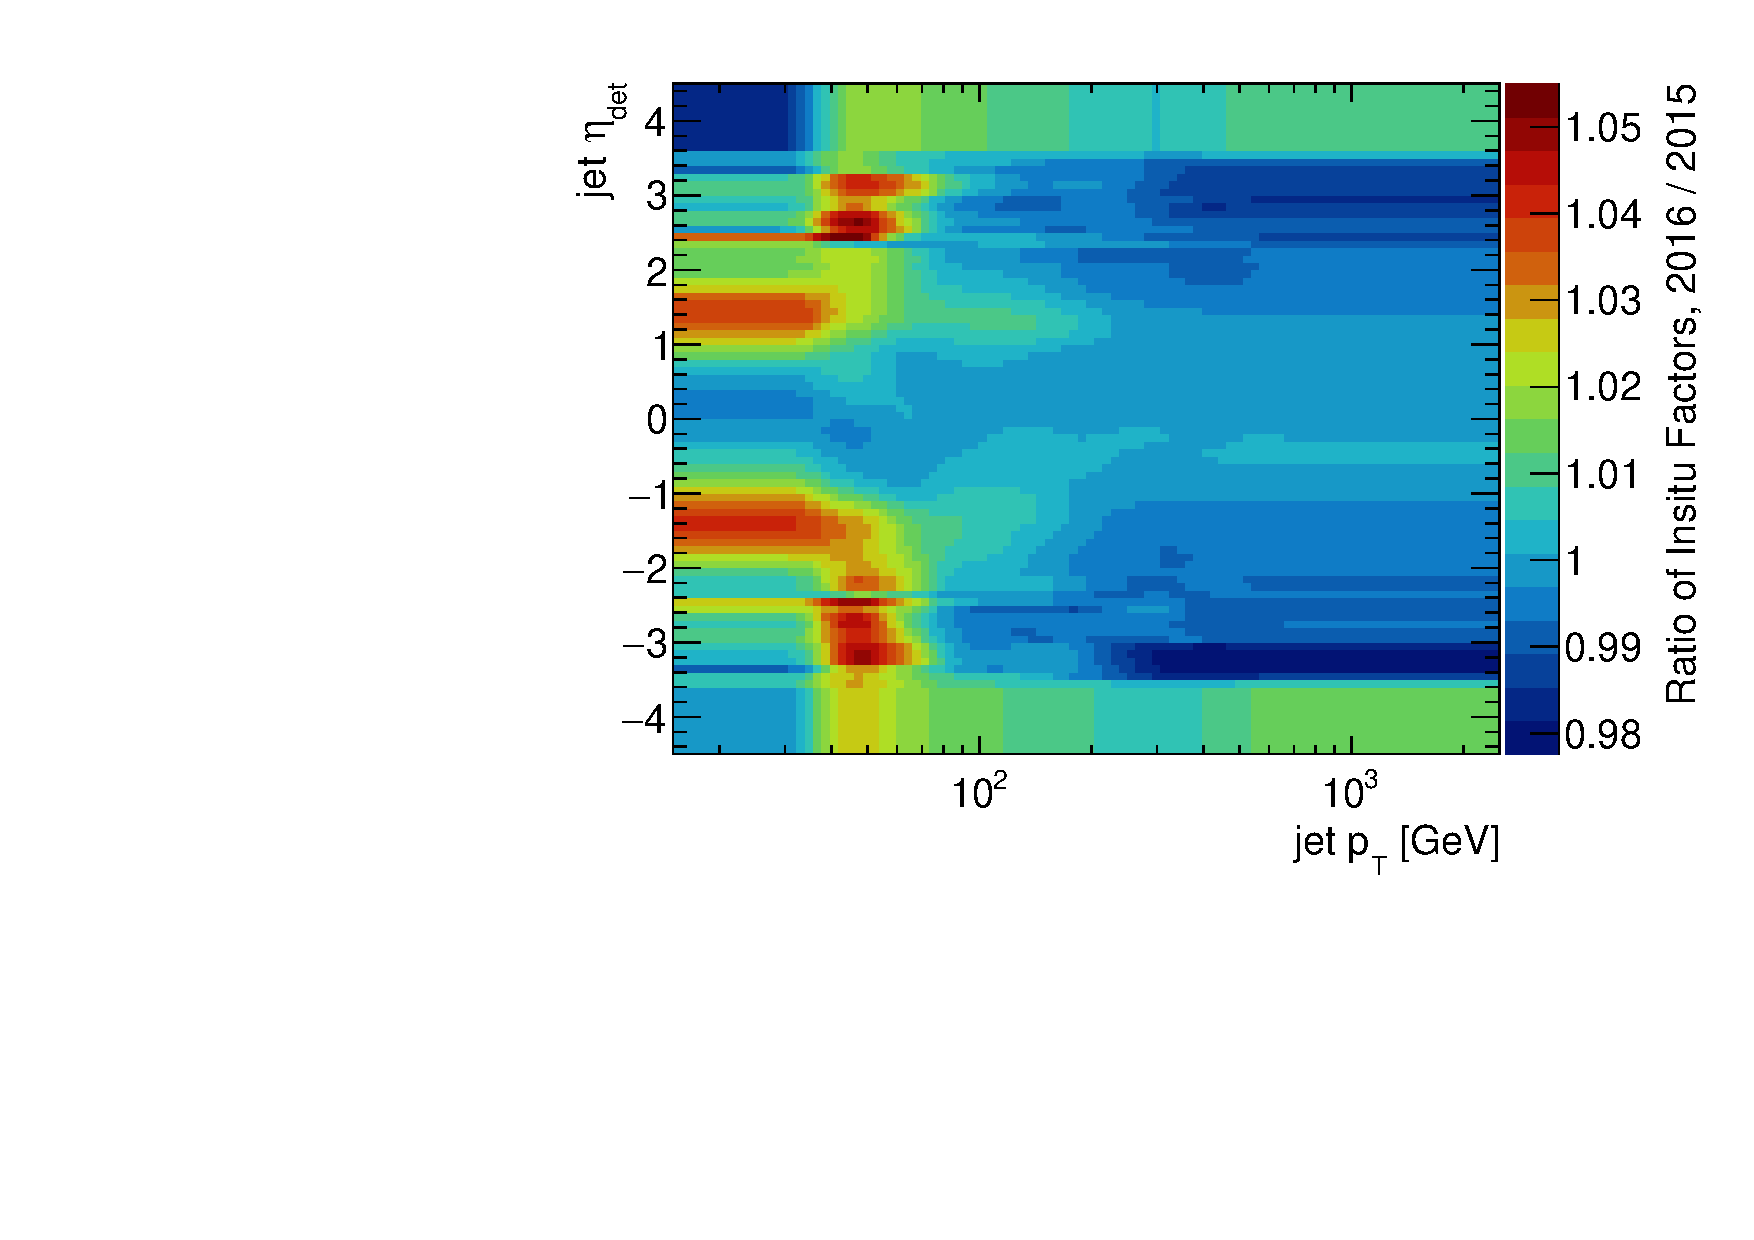
\includegraphics[width=0.45\textwidth]{../InsituComparison/CompareEtaInterCcalibration.pdf}
		\label{fig:insituEtaComp}
	}
	\subfloat[]{
		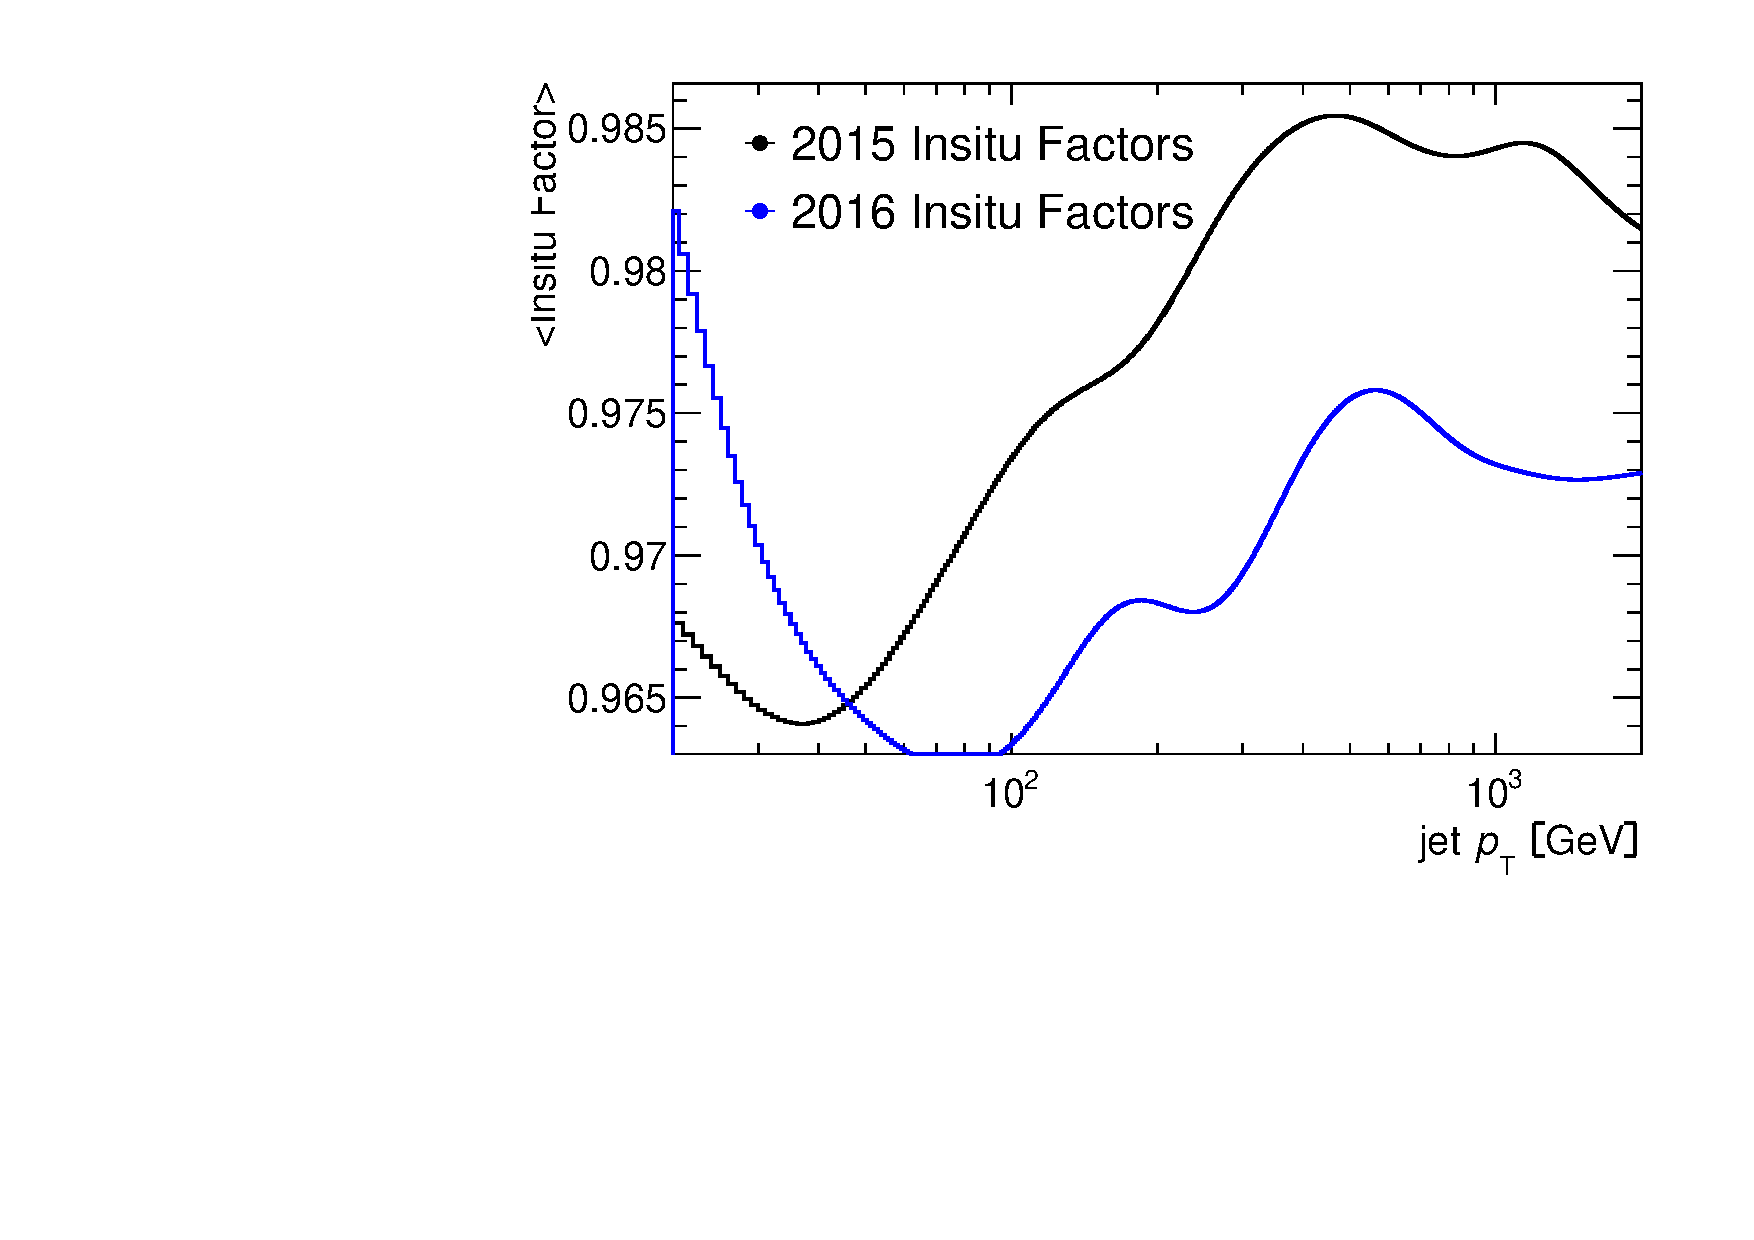
\includegraphics[width=0.45\textwidth]{../InsituComparison/CompareSummary.pdf}
		\label{fig:insituCompSummary}
	}
	\caption{A comparison of the \textit{in situ} factors from 2015 data to 2016 data. Left: the \textit{in situ} factors in 2016 are divided by those in 2015, as a function of $\eta$ and $\pt$. Right: the \textit{in situ} factors for each year are averaged over $\eta$ and displayed as a function of $\pt$, showing a substantial difference.}
	\label{fig:insituComp}
\end{figure}

Jet transverse momentum is then compared to vector boson transverse momentum using the quantity $x_{\text{J}}^{\text{ref}}$, as defined in equation \ref{eq:xjref}, binned by jet pseudorapidity. The projection onto the antiparallel is intended to account for soft radiation from the jet that is (potentially) missed by the jet finding algorithm.
\begin{equation}
	x_{\text{J}}^{\text{ref}} = \frac{\pt^{\text{jet}}}{\pt^{\text{V}} \cos{\Delta\phi}}
	\label{eq:xjref}
\end{equation}
Because the jet response is $\pt$-dependent, and the cross-calibration factors depend on $\eta_{\text{det}}^{\text{Jet}}$, $x_{\text{J}}^{\text{ref}}$ has been averaged as a function of $\pt^{\text{ref}}$ and $\eta_{\text{det}}^{\text{Jet}}$. 

Additionally, a hadronic background subtraction procedure is also performed exclusively in the $\gamma$-tagged events. Because the photon purity has been previously studied in this collision system, contributions from background photons can be estimated. Measured distributions of reconstructed photons marked as loose-non-tight (LNT) can be subtracted as a background, under the assumption that the shape of the loose-non-tight distribution matches the background shape:
\begin{equation}
	\frac{dN_{\text{tight}}}{dx^{\text{ref}}_{\text{J}}}\bigg{|}_{\text{bkg}} = (1 - p) \times \frac{N_{\text{tight}}}{N_{\text{LNT}}} \times \frac{dN_{\text{LNT}}}{dx^{\text{ref}}_{\text{J}}}
	\label{eq:bkg}
\end{equation}
 where $p$ is the photon purity \cite{ATL-COM-PHYS-2017-999}.
 
% shown in Figure \ref{fig:purity}.
%
% \begin{figure}[htbp]
% 	\centering
%	\includegraphics[width=\textwidth]{figures/sideband_purity_pt_combo_sys0.pdf}
%	\caption{Inclusive photon purity derived in MC.}
%	\label{fig:purity}
%\end{figure}

For the jets at central rapidity $\left|\eta_{\text{det}}^{\text{Jet}}\right| < 1.2$, the results can be seen in Figure \ref{fig:xjref_pT_central}. In addition to plotting the mean $x_{\text{J}}^{\text{ref}}$, a quadratic in $\text{log}(\pt^{\text{ref}})$ is fitted to the data-to-MC ratio to account for bin-to-bin statistical variation, using the form in Equation \ref{eq:fit} below. To reduce correlation of the fit parameters, an orthogonal Chebyshev basis is used. A 95\% confidence interval from the fit is also shown. For $\left|\eta_{\text{det}}^{\text{Jet}}\right| > 1.2$, the results are similarly in Figure \ref{fig:xjref_pT_forward}.

\begin{equation}
	%f \left(\log \pt^{\text{ref}}\right) = f (x) = a_0 + a_1\left(\frac{\log \pt^{\text{ref}} - \log \pt^{\text{avg}}}{\log \Delta\pt}\right)  + a_2\left(2\left(\frac{\log \pt^{\text{ref}} - \log \pt^{\text{avg}}}{\log \Delta\pt}\right) ^2 - 1\right)
	%f \left(\log \pt^{\text{ref}}\right) = f (x) = a_0 + a_1x  + a_2\left(2x^2 - 1\right)
	f (x) = a_0 + a_1x  + a_2\left(2x^2 - 1\right)
	\label{eq:fit}
\end{equation}


%\subsection{Derivation of additional uncertainties}
%For jets in each $\eta$ bin, the additional systematic uncertainty from the cross calibration can be estimated as the change in $\pt^{\text{jet}}$ required to match the data to MC. Since $p_{\text{T}}^{\text{ref}}$ is plotted on the horizontal axis, this can be done by taking the root-mean-square of the quantity $\sigma \left(\pt^{\text{ref}}\right) = \pt^{\text{ref}} \times\left( \left< x_{\text{J}}^{\text{ref}} \right>_{\text{data}} - \left< x_{\text{J}}^{\text{ref}} \right>_{\text{MC}} \right)$ as a function of $\pt^{\text{jet}}$.

\begin{figure}[htbp]
	\centering
	\subfloat[]{
		\includegraphics[width=0.45\textwidth]{figures/gamma_jet_PA_iEta_combined.pdf}
		\label{fig:g_PA_pT_central}
	}
	\subfloat[]{
		\includegraphics[width=0.45\textwidth]{figures/gamma_jet_PB_iEta_combined.pdf}
		\label{fig:g_PB_pT_central}
	} \\
	\subfloat[]{
		\includegraphics[width=0.45\textwidth]{figures/z_ee_jet_PA_iEta_combined.pdf}
		\label{fig:zee_PA_pT_central}
	}
	\subfloat[]{
		\includegraphics[width=0.45\textwidth]{figures/z_ee_jet_PB_iEta_combined.pdf}
		\label{fig:zee_PB_pT_central}
	} \\
	\subfloat[]{
		\includegraphics[width=0.45\textwidth]{figures/z_mumu_jet_PA_iEta_combined.pdf}
		\label{fig:zmumu_PA_pT_central}
	}
	\subfloat[]{
		\includegraphics[width=0.45\textwidth]{figures/z_mumu_jet_PB_iEta_combined.pdf}
		\label{fig:zmumu_PB_pT_central}
	}
	\caption{$V$ + jet average $x_{\text{J}}^{\text{ref}}$ in both period A and period B collisions as a function of $p_{\text{T}}^{\gamma}$ for jets near mid-rapidity. Top row: $\gamma$ + jet events, middle row: $\Zboson\rightarrow\ee$ + jet events, \& bottom row: $\Zboson\rightarrow\mumu$ + jet events. Left column: period A collisions, right column: period B collisions.}
	\label{fig:xjref_pT_central}
\end{figure}

\begin{figure}[htbp]
	\centering
	\subfloat[]{
		\includegraphics[width=0.45\textwidth]{figures/gamma_jet_PA_iEta_uncombined.pdf}
		\label{fig:g_PA_pT_forward}
	}
	\subfloat[]{
		\includegraphics[width=0.45\textwidth]{figures/gamma_jet_PB_iEta_uncombined.pdf}
		\label{fig:g_PB_pT_forward}
	} \\
	\subfloat[]{
		\includegraphics[width=0.45\textwidth]{figures/z_ee_jet_PA_iEta_uncombined.pdf}
		\label{fig:zee_PA_pT_forward}
	}
	\subfloat[]{
		\includegraphics[width=0.45\textwidth]{figures/z_ee_jet_PB_iEta_uncombined.pdf}
		\label{fig:zee_PB_pT_forward}
	} \\
	\subfloat[]{
		\includegraphics[width=0.45\textwidth]{figures/z_mumu_jet_PA_iEta_uncombined.pdf}
		\label{fig:zmumu_PA_pT_forward}
	}
	\subfloat[]{
		\includegraphics[width=0.45\textwidth]{figures/z_mumu_jet_PB_iEta_uncombined.pdf}
		\label{fig:zmumu_PB_pT_forward}
	}
	\caption{$V$ + jet average $x_{\text{J}}^{\text{ref}}$ in both period A and period B collisions as a function of $p_{\text{T}}^{\gamma}$ for jets away from mid-rapidity. Top row: $\gamma$ + jet events, middle row: $\Zboson\rightarrow\ee$ + jet events, \& bottom row: $\Zboson\rightarrow\mumu$ + jet events. Left column: period A collisions, right column: period B collisions.}
	\label{fig:xjref_pT_forward}
\end{figure}

%-------------------------------------------------------------------------------
\section{Conclusion}
\label{sec:conclusion}
%-------------------------------------------------------------------------------

The jet energy scale corrections for anti-$k_{\text{T}}$ $R=0.4$ jets has been derived in $\SI{8.16}{\TeV}$ \textit{p}+Pb collisions. A new cross-calibration configuration with the 2016 \textit{in situ} factors and 2015 cross-calibration factors has been created and tested for applicability in the newer data. At mid-rapidity, only minor deviation is observed and is generally covered by errors, but larger deviations exist in the $\pt$ balance at forward and backward rapidities.  


%-------------------------------------------------------------------------------
% If you use biblatex and either biber or bibtex to process the bibliography
% just say \printbibliography here
\clearpage
\printbibliography
% If you want to use the traditional BibTeX you need to use the syntax below.
% \bibliographystyle{obsolete/bst/atlasBibStyleWithTitle}
% \bibliography{pPbJetCalibrationNote,bib/ATLAS,bib/CMS,bib/ConfNotes,bib/PubNotes}
%-------------------------------------------------------------------------------

%%-------------------------------------------------------------------------------
%% Print the list of contributors to the analysis
%% The argument gives the fraction of the text width used for the names
%%-------------------------------------------------------------------------------
%\clearpage
%The supporting notes for the analysis should also contain a list of contributors.
%This information should usually be included in \texttt{mydocument-metadata.tex}.
%The list should be printed either here or before the Table of Contents.
%\PrintAtlasContribute{0.30}


%%-------------------------------------------------------------------------------
%\clearpage
%\appendix
%\part*{Appendices}
%\addcontentsline{toc}{part}{Appendices}
%%-------------------------------------------------------------------------------

%In an ATLAS note, use the appendices to include all the technical details of your work
%that are relevant for the ATLAS Collaboration only (e.g.\ dataset details, software release used).
%This information should be printed after the Bibliography.

\end{document}
